% This is lnbip.tex the demonstration file of the LaTeX macro package for
% Lecture Notes in Business Information Processing from Springer-Verlag.
% It serves as a template for authors as well.
% version 1.0 for LaTeX2e
%
\documentclass[lnbip]{svmultln}
%
\usepackage{makeidx}  % allows for indexgeneration
\usepackage{graphicx}
% \makeindex          % be prepared for an author index
%
\newcommand{\mari}[1]{\footnote{MARI: #1}}
\begin{document}
%
\mainmatter % start of the contribution
%
\title{Prototypes are forever\\
  Evolving from a prototype project\\ to a full-featured system}
%
\titlerunning{Prototypes are
  forever} % abbreviated title (for running head)
% also used for the TOC unless \toctitle is used
%
\author{Hugo Corbucci\inst{1} and Mariana V. Bravo \inst{1} and
  Alexandre Freire\inst{1}}
%
\authorrunning{Hugo Corbucci et
  al.}  % abbreviated author list (for running head)
%
%%%% list of authors for the TOC (use if author list has to be
%%%% modified)
\tocauthor{Hugo Corbucci and Mariana V. Bravo and Alexandre Freire}
%
\institute{Agilbits, Sao Paulo, Brazil,\\
  \email{{hugo,marivb,freire}@agilbits.com.br}}

\maketitle % typeset the title of the contribution
% \index{Ekeland, Ivar} % entries for the author index
% \index{Temam, Roger} % of the whole volume
% \index{Dean, Jeffrey}

\begin{abstract} % give a summary of your paper

  % TODO Abstract
  This paper shows our experience evolving a prototype to a full
  featured project.
  % please supply keywords within your abstract TODO Keywords
  \keywords {prototype, agile methods, }
\end{abstract}
%
\section{Introduction}

Prototyping is an activity that most developers have heard about. Fred
Brooks mentioned it in The Mythical Man-Month~\cite{Brooks1975} as one
of the best ways to provide a quick view of a feature to the clients
or users to help them make a choice. Dynamic System Development Method
(DSDM)~\cite{DSDM} is heavily based on prototyping and other agile
methods also adopt many ideas related to this concept like
spikes~\cite{XP} in the Extreme Programming exploration
phase. However, those who have had some experience with this practice
feel uncomfortable with it\cite{quem disse? esse tipo de afirmação é
  sempre bom ter uma citação, já apanhei bastante sobre isso.  ale}.

Successful software prototypes look very much like complete features
given a certain execution path. Therefore it is common that the
customers are so satisfied that they want to integrate the prototypes
to the working system and move on. The problem is that prototypes are
frequently created in a ``quick and dirty'' fashion and the result is
not adequate to be incorporated in a full-featured system. Yet it is
quite hard to explain this fact to the stakeholders who usually do not
want to invest any more money in this ``already working'' feature. The
consequence is that they switch priorities, focus developer work
efforts on other parts of the system and leave the rough prototype
lost within the code base. Months or years later, the prototype has
become a part of the system but is filled with bugs, unhandled corner
cases and, frequently, crappy code. Nobody remembers what it was
supposed to do or whether it is really important. Maintainability gets
deeply affected and developers get that natural and unpleasant
I-told-you-so feeling. %TODO trauma?

Developers that have been through the pain of maintaining those dirty
prototypes are no longer enthusiastic to work with prototypes. If they
have to, they make it so that there will be absolutely no way to
integrate the prototype to the existing system by either using a
different platform, language or even creating prototypes in other
medias. That inflexibility can reduce the ability of responding to
changes quickly and therefore harm the clients' interests.

This paper presents how a four-people collocated team managed to start
a prototyping project and evolve it naturally to a full-featured
application.  We have organized this experience report following the
chronological order of the project's evolution. Section
\ref{sec:start} will present the project as it was first introduced to
the development team. Section \ref{sec:working} presents the work
process established by the team to create the software based on
prototypes. After some time, the team felt that the customer needed a
full featured application, we describe this change in Section
\ref{sec:changes}. The following section (Section \ref{sec:adapting})
shows how the team adapted to change to evolve the prototype to a
production ready application. Finally Section \ref{sec:nowadays}
presents the current status of the project. Section \ref{sec:conclusion} concludes with a
summary of practices that were useful to go through this experience
without much pain.

\section{Starting the project}
\label{sec:start}

Back in March 2008, our company was hired to do some consulting for
one of the largest movie producing companies in Brazil. The client had
a great idea for a software to write movie scripts but had absolutely
no knowledge about software development.  He wanted to mature the idea
and understand how much investment it would take to turn it into
working software in order to establish his business plan. The
company's job at the time was to scout the market, discover
competitors and provide an estimation of the work needed to develop
the client's idea.

For such work, one consultant was assigned to understand what were the
client's needs and desires and two developers were asked to analyze
the existing script writing programs and evaluate the possible
development paths. After about 3 weeks of consulting and studies, the
team handed a deck full of story cards with two estimates each, based
on the use of two possible platforms. The first platform was an
existing open source software with several features and a copy-left
license; the second one was an Eclipse Rich Client Application
developed from scratch using Eclipse's open source framework.

This initial estimation suggested that a four people team dedicating 4
daily work hours to the project would be able to build a working
prototype of each feature described in about nine months of
development using the existing open source software and about one year
using Eclipse's platform. The open source solution had the advantage
to provide full functionality of several other features. For a
complete system, the estimation was well over 2 years of work on the
Eclipse version and about a year and a half for the open source one.

After some discussion, the client opted for the Eclipse based solution
due to the license restriction of the open source one which conflicted
with his business plan. He also chose to develop only a prototype of
the idea since 2 years seemed like a too heavy investment for him
alone.

After the exploration phase, the consulting contract ended and a new
negotiable scope contract\cite{tem citação pra esse tipo de contrato?}
with emphasis on development effort was established. This new contract
established a team of 4 developers working with open scope that would
be negotiated monthly, providing 160 hours of work each month. It
specifically stated that the developers would work on pairs all the
time and that the developed system should have automated tests to the
production code.

% Initial priority of the stories, taken from Paulo's spreadsheet:
% Phase 1 => read TXT / separate and number act, sequence and scenes /
% read and show touch / read and show "thread" (characters) / "vision"
% (script tree) / zoom / add notes (summary) / edit touch and
% "threads" Phase 2 => create script from scratch / edit script text /
% "mundo das fichas" Phase 3 => read RTF / read and export FDR

The features initially presented to the team were grouped by the
client into 3 priority groups. The first group contained all features
most critical to the client, the ones that would allow him to
experiment with his ``big idea''. The second one comprised of some
features already present in most script editors in the market, such as
editing the script text itself. Most features in this second group
were in fact epics. The third group contained only features to read
and export to different file formats, such as those used by competitor
programs.

The project's goal was to create a high visual fidelity prototype with
mostly faked or simplified features from the first group. The client
would use this prototype to present his ideas to investors by October
2008. This meeting would either boost the project's development to a
full featured system if the investors liked the idea or end its
development in case they rejected it.

That was the team's vision of the project when the development
begun. A short seven months project whose fate would be decided by its
capacity to impress investors. Therefore, the main goal was to provide
support for the client's demonstration to ensure the project's growth
and success. The next section (Section \ref{sec:working}) describes
how the team organized itself to achieve this goal.

\section{Prototyping phase}
\label{sec:working}

Given the project's objective, the customer always prioritized new
features considering only one specific usage scenario. This meant
that, for most features, there were several cases which the team was
asked \textbf{not} to handle. Regarding the source code, it meant
that no verification or validation was written and the prototype would
crash if the user did not behave as expected. We also incorporated
several spikes as permanent solutions and did not handle a fair amount
of exceptions, ignoring errors.

The team knew since the beginning that the client would change his
mind over time. After all, it was partly to better understand his idea
and its applicability that he wanted to build this prototype. This
meant that features would be developed to later be thrown away while
code produced only for a quick spike was going to become part of the
system. Therefore, since the beginning the team invested on design,
automated tests and refactoring, just enough to keep the system
flexible to receive the next changes. The team also made it clear for
the client that he would need some work done on features after he
accepted them in order to polish the work.

The first few iterations went quite smooth, developing features from
the first phase which involved importing a script in a text-only
format, providing a simple way to mark text with meta-data and a way
to manipulate and visualize this data. For these first features, it
was easy to avoid inconsistencies since there were not many business
rules involved.% Problems started to appear on later iterations once we
%needed to save changes and handle script modifications with more
%complex business rules.
%TODO \mari{ainda nao gosto dessa frase...}

% TODO Mari quer rever esse paragrafo, parece historicamente incorreto
% as features do "grupo 1" estavam "prontas" (prototipadas), mas ele
% quis entrar no editor, que estava no grupo 2.
Meanwhile, the client's demonstration script was evolving as the prototype did and the team was able to use conditionals as needed to ignore cases he would not enter in during his presentation to investors. By October 2008, the main features from the first group were ready for demonstration, but not finished and polished for real use. 

Even so, the client did not feel completely confident to present the software to the investors because he realized that the program still lacked an important 

he had discovered and prioritized new features that he felt were important but that were still incipient in the prototype. However, he started to make contact with a few people to schedule a meeting by the end of November 2008 or start of December 2008. Those dates became our new deadline until which all efforts should be focused on making those incipient features available for the demonstration.

At this point, the pressure for polishing the new features increased
since the project's fate would be decided at the demonstration and it
was close! The customer wanted the team to ignore corner cases, speed
up delivery and ensure the demonstration would run smoothly. The
excitement from the important presentation to other people (only our
one client and us had seen the software so far) was a strong
motivation for the development team to deliver all features the client
had asked for. Yet, despite unit testing and pair programming being
mandatory rules on the team, the general will to quickly deliver the
features decreased the code quality considerably.

Things were getting quite unpleasant
%TODO \mari{mari tb não gosta do  "unpleasant"}
from a development perspective but since the client
satisfaction was still high, there was little that could be
done. However, external interference was about to change a bit the
situation. Section \ref{sec:changes} will explain how the project got
affected and what new direction those changes pointed to.

\section{Changing the rules}
\label{sec:changes}

December 2008 came and went without any meeting. The company that
the client was in contact with had just been acquired by another one
so any project presentation was useless until things settled
down. That news pushed the deadline away for another 3 or 4 months at
least. Along with this news came the information that the client had
formed a dramaturgy experts group to help him better understand how to
structure the application.

This new context relieved a 4 months pressure of upcoming deadline
over a team which was beginning to feel the burden of unhandled
technical debt. All members of the development team agreed that the
code was getting complex and the quality was decreasing which was
affecting productivity and speed. The software was now going to have a
set of beta testers and it needed to perform decently to allow the
users to suggest improvements for it.

The general feeling was that the project was no longer aimed at a
simple presentation to investors. It was softly switching to a more
elaborate end user oriented application. The current development
approach would not be able to support this new use of the system. The
change had to be clear to the client so that development efforts would
be directed to address this new way of working.

The warnings came quickly from the dramaturgy study group. They
started having trouble with several known and unknown corner cases,
unexpected behaviors and just plain old bugs. The client noticed this
and decided it was time to invest more in usability and user
experience. The team made it clear that this would also mean less new
features delivered and even managed to dedicate a whole iteration to
refactoring.

At this point, the client started to understand the dilemma that the
developers had felt so far. How to keep a good rhythm of new feature
delivery and still cover most use cases of existing features? Another
critical issue in the software was that, so far, most features were
aimed at visualization and insertion of meta data in the scripts, but
users were claiming for basic text editing features that had been
ignored so far.

The team estimated that to have an editor with the basic functionality
expected by the client would take at least three full iterations. This
was not welcomed by the client since it would mean that no new
features would be added until the moment when he would possibly be
able to show the software to investors. So he took another action
which indicated changes in the business plan of the project.  The
development team suggested that another team could work on text
editing features parallel to them so that they could continue working
on the new features he wanted.

After some research we discovered an open source Eclipse Rich Client
WYSIWYG (What You See Is What You Get) HTML
editor\footnote{\url{http://onpositive.com/richtext/} - Last accessed
  on 20/02/2010}. The editor relied on a reimplementation of Eclipse's
StyledText component which is responsible for rendering text within
Eclipse editors. This component was close enough from the one we
needed to implement, having some of the functionality our client
wanted on our application. So the client outsourced the development of
this underlying infra-structure to this open source project as a way
to keep the new-feature delivery velocity while attending the users'
requests.

Meanwhile, the development team was concerned with the increasing
complexity so they started to track some data from the source
code. The first metrics was the amount of \texttt{FIXME},
\texttt{TODO} and \texttt{XXX} marks in the code. As previously
mentioned, the development team added those marks everywhere they felt
a corner case or a behavior existed but was not handled. Each mark had
a small comment associated and the kind of the mark determined the
criticality of the problem. Figure \ref{fig:TODOs} shows the evolution
of those marks during the project.

\begin{figure}[hbt]
  \centerline{
    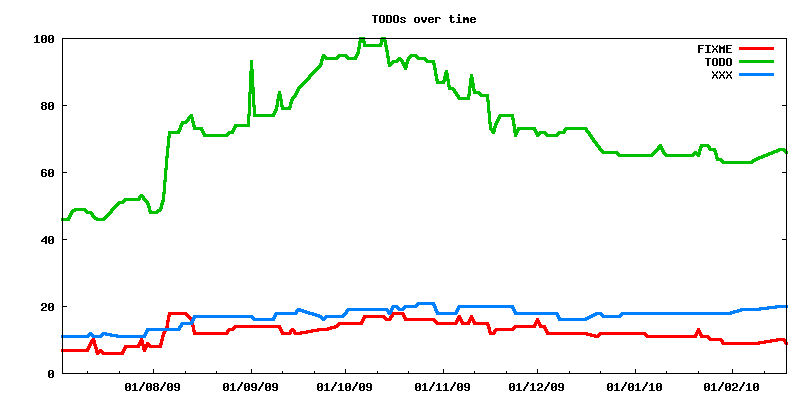
\includegraphics[width=120mm]{TODOs.png}
  }
  \caption{Evolution of FIXME, TODO and XXX marks in the source code}
  \label{fig:TODOs}
\end{figure}

Notice that the first data collection of those marks is dated for mid
July 2009. It took the team some time to consider this metric was
important enough to be automatically tracked and generated. To
consciously acknowledge that the team needed to track complexity was
step one to adapt to the new direction. The next section will present
other practices that allowed to handle this shift.

\section{Adapting to the new rules}
\label{sec:adapting}

\begin{figure}[hbt]
  \centerline{
    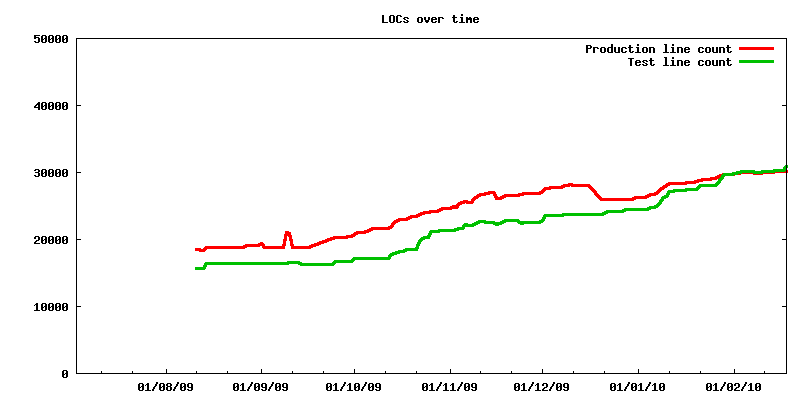
\includegraphics[width=120mm]{LOCs.png}
  }
  \caption{Evolution of production lines of code and test lines of
    code}
  \label{fig:LOCs}
\end{figure}

While the amount of \texttt{TODO} marks was fairly high, the team
still had to develop new prototyped features and therefore they
accepted to just track it and try to keep it under control. While this
gave the team some idea of code complexity, it did not help in showing
if this complexity was being tamed by tests.

By the beginning of August 2009, the client decided that it was
important for him to be able to see the evolution of the work done by
the Russian team and he decided to have two editors available on the
application. The first one was Eclipse's original one and the second
one was based on the new outsourced component. At this point, a major
code duplication was performed since features were duplicated and the
goal was to eliminate our old editor. The result was a huge increase
in the marks tracking as well as an increase in lines of code and the
team suspected tests were not following. A very simple script was
written to count the lines of production code and test code. Figure
\ref{fig:LOCs} shows how both metrics evolved over time. It starts at
the same date as Figure \ref{fig:TODOs} to facilitate comparisons.

As for the \texttt{TODO} metric, the lines of code showed the team a
little issue regarding testing but it was not addressed immediatly. It
was well known that the code was not highly covered since there were
no User Interface (UI) tests and quite a few feature were related to
the way data was shown to the user. However, the team had a feeling
that the effort to test the controller and model would have produced
more test than code.

By this time, the customer started to mention again the presentation
to the investors. It had been quite some time in the project now and
he was feeling he had spent enough money and needed some external
investment. Therefore the old investor meeting pressure installed
itself within the team and the deadline was, again, the end of the
year. The goal was to quickly integrate the outsourced component and
tune a few features to the so expected meeting.

By the time the team was understanding the outcomes of those issues,
the code had reached a critical situation. \texttt{TODO} marks were
amazingly high and distance between tests and code was at its higher
level. The work was being roughly divided in three: fixing bugs,
implementing new features and integrating the outsourced component. By
this time, the team also suffered the loss of a member who was
required in a full time consulting work. The team went from two pairs
to one pair and an extra person and the velocity decreased.

Figure \ref{fig:InstanceOfs} shows yet another complexity tracker
developed by the team. Counting the amount of \texttt{instanceof} Java
reserved word led the team to understand the level of special cases
unfactored in the code. Although Eclipse's framework required a few of
those, some of them were avoidable and the team felt reducing this
number would lead to a more factored code.

\begin{figure}[hbt]
  \centerline{
    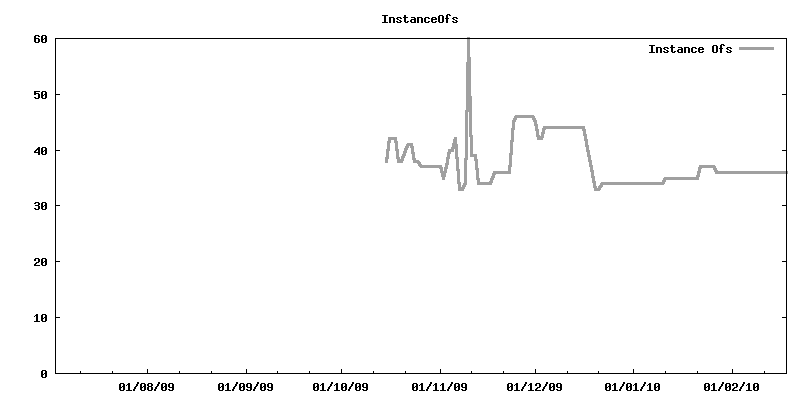
\includegraphics[width=120mm]{InstanceOfs.png}
  }
  \caption{Evolution of instanceof in the code }
  \label{fig:InstanceOfs}
\end{figure}

Curiously, as for the two previous metrics, the effect of tracking the
number of \texttt{instanceof} was not immediate. More interestingly
than that, in a short time span, having the metric did not stop it
from getting worse. In the rush to produce the features, the team was
becoming reckless with code quality.  Something had to be done or the
project was going to become impossible to maintain and the client's
demonstration would surely suffer from it.

With three persons working by the end of the year to match a two pairs
velocity and reducing complexity, the team had to calm down, step back
and rethink about agile values. Section \ref{sec:nowadays} presents
the resolutions the team adopted and their impact on the current
version of the system.

\section{Current status}
\label{sec:nowadays}

December arrived and it was time to accept a full integration of the
outsourced component and a throw away of the team's first
solution. Along with this came a serious decrease in \texttt{TODO}
marks, \texttt{instanceof}s and lines of production code as a
considerable duplication was erased. By that time, the team was
largely working with just two persons paring full time since the third
developers was involved in other projects and hardly managed to pair.

The team decided it should profit from that fact and decided to
institute a merciless refactoring policy. No matter how small or how
big the refactoring was, it had to be done and it was to be included
as a regular part of each task and not as a separated task. Corner
cases were not to be left handled and any unsupported work was to log
its execution to the application error log. The impact of those
policies was fairly clear by the end of the month. All metrics had
improved and more bugs were being listed by the development team.

The month passed and no meeting was scheduled. The famous deadline
was, once again, a myth. With code quality increasing, \texttt{TODO}
marks decreasing, test code improving and bugs being caught by the
development team (instead of the users), the team felt an extra
developer would help increase velocity and so started to train him to
join the team in January. With the insertion of this new member in the
team, some work was performed on another platform which led to the
discovery of a serie of platform specific bugs. The general feeling
was that the client was getting ready to wrap up the project since he
was quite happy with the software and was considering he invested too
much already on this idea.

However, in the next meeting, the client presented an official hired
beta tester that was going to support the team improve the usability
of the system. They also presented the team with a load of new
features and usability improvements that they wanted to have done. The
client also mentioned that he thinking seriously about dropping the
quest for investors and releasing the product by himself. In order to
do so, bugs needed to be eliminated. Any bugs found immediately gained
the highest priority and should be solved in some way as soon as
possible.

With this new policy, the team started to find problems with the
existing features because some cases conflicted. Those issues reported
to the customer led him study and analyse more his business model and
the rules evolved so far. Thanks to the experience that the client had
accumulated so far in the project, he allowed himself to experiment a
few solutions until he felt more comfortable with the way features
worked allowing him to seek consistency, conceptual integrity and the
certainty that other choices were not as good as the one he had made.

\section{Conclusion}
\label{sec:conclusion}

Team's effort to keep tests level (ignoring known issues not solved).

Refactor tests.

Refactor prototypes (their code must be good).

%
% ---- Bibliography ----
%
\begin{thebibliography}{5}

\bibitem{Brooks1975} Brooks Jr., F.P.: The Mythical Man Month: Essays
  on Software Engineering. Addison-Wesley (1975)

\bibitem{DSDM} DSDM Consortium: DSDM: Business Focused
  Development. Addison-Wesley (2002)

  % ale: achei que era uma boa ter mais referências sobre
  % prototipos. eu tirei essa história de prototipos de alta
  % fidelidade visual ou alta fidelidade funcional de uma apresentação
  % que vi sobre UX e prototipagem de interface lá na locaweb, no
  % scholar.google achei isso aqui:

  % http://74.125.155.132/scholar?q=cache:ezGZKBBRVhwJ:scholar.google.com/+software+prototype&hl=pt-BR&as_sdt=2000

  % http://www.imamu.edu.sa/Scientific_selections/abstracts/Documents/A%20Systematic%20Look%20At%20Prototyping.pdf

\end{thebibliography}
%
\end{document}
